%%%%%%%%%%%%%%%%%%%%%%%%%%%%%%%%%%%%%%%%%%%%%%%%%%%%%%%%%%%%%%%%%%%%%%
% LaTeX Example: Project Report
%
% Source: http://www.howtotex.com
%
% Feel free to distribute this example, but please keep the referral
% to howtotex.com
% Date: March 2011 
% 
%%%%%%%%%%%%%%%%%%%%%%%%%%%%%%%%%%%%%%%%%%%%%%%%%%%%%%%%%%%%%%%%%%%%%%
% How to use writeLaTeX: 
%
% You edit the source code here on the left, and the preview on the
% right shows you the result within a few seconds.
%
% Bookmark this page and share the URL with your co-authors. They can
% edit at the same time!
%
% You can upload figures, bibliographies, custom classes and
% styles using the files menu.
%
% If you're new to LaTeX, the wikibook is a great place to start:
% http://en.wikibooks.org/wiki/LaTeX
%
%%%%%%%%%%%%%%%%%%%%%%%%%%%%%%%%%%%%%%%%%%%%%%%%%%%%%%%%%%%%%%%%%%%%%%
% Edit the title below to update the display in My Documents
%\title{Project Report}
%
%%% Preamble
\documentclass[paper=a4, fontsize=11pt]{scrartcl}
\usepackage[T1]{fontenc}
\usepackage{fourier}

\usepackage[english]{babel}															% English language/hyphenation
\usepackage[protrusion=true,expansion=true]{microtype}	
\usepackage{amsmath,amsfonts,amsthm} % Math packages
\usepackage[pdftex]{graphicx}	
\usepackage{url}
\usepackage[titletoc,title]{appendix}
\usepackage[boxruled ]{algorithm2e}
\usepackage{listings}
\usepackage{bm}


%%% Custom sectioning
\usepackage{sectsty}
\allsectionsfont{\centering \normalfont\scshape}


%%% Custom headers/footers (fancyhdr package)
\usepackage{fancyhdr}
\pagestyle{fancyplain}
\fancyhead{}											% No page header
\fancyfoot[L]{}											% Empty 
\fancyfoot[C]{}											% Empty
\fancyfoot[R]{\thepage}									% Pagenumbering
\renewcommand{\headrulewidth}{0pt}			% Remove header underlines
\renewcommand{\footrulewidth}{0pt}				% Remove footer underlines
\setlength{\headheight}{13.6pt}


%%% Equation and float numbering
\numberwithin{equation}{section}		% Equationnumbering: section.eq#
\numberwithin{figure}{section}			% Figurenumbering: section.fig#
\numberwithin{table}{section}				% Tablenumbering: section.tab#


%%% Maketitle metadata
\newcommand{\horrule}[1]{\rule{\linewidth}{#1}} 	% Horizontal rule

\title{
		%\vspace{-1in} 	
		\usefont{OT1}{bch}{b}{n}
		\normalfont \normalsize \textsc{Braket Technologies Technical Report} \\ [25pt]
		\horrule{0.5pt} \\[0.4cm]
		\huge Bearing Angle Errors Due to Pipe Background \\
		\horrule{2pt} \\[0.5cm]
}
\author{
		\normalfont 								\normalsize
        Braket Technologies\\[-3pt]		\normalsize
        \today
}
\date{}


%%% Begin document
\begin{document}
\maketitle
\section{Introduction}
Scott.  Maybe you can write something in here that sets the context for this work.  The type of instrument used, the circumstances that triggered this work, etc.

\section{The Rest of the Paper}
Scott write this.

Here is sin phi model.
measurement is the sum of the two
drop into phasor
define max error
compute bearing correction for exactly knows sig/back
talk stats





\begin{appendices}
\section{Estimating the Bearing Correction}
\subsection{The Bearing Correction}
The signal measured within the pipe will vary as a function of angle.  We can break down the source of this signal into two components.  The first component we will call the ``cable signal.''  This is the signal variation caused by the presence of the cable attached to the outside of the pipe.  The second component we will call the ``background signal,'' which arises from all other sources of angular asymmetry in the system.  This is thought to be dominated by imperfect centering of the instrument within the pipe.

\par We model both the background and cable signals as if they were sinusoidal function.  Figure \ref{fig:sigs_vs_bearing} shows a model we will use as an example for describing our analysis.  In this model, the background signal is one quarter the amplitude of the cable signal and it is offset in angle by 135 degrees.  The instrument will measure the sum of these two signals, which, of course, will have a different amplitude and phase than either of is constituent signals.

\begin{figure}
  \caption{An Example Model.  The background signal is one quarter the amplitude of the cable signal, and has a 135 degree offset in bearing.}
  \label{fig:sigs_vs_bearing}
  \centering
  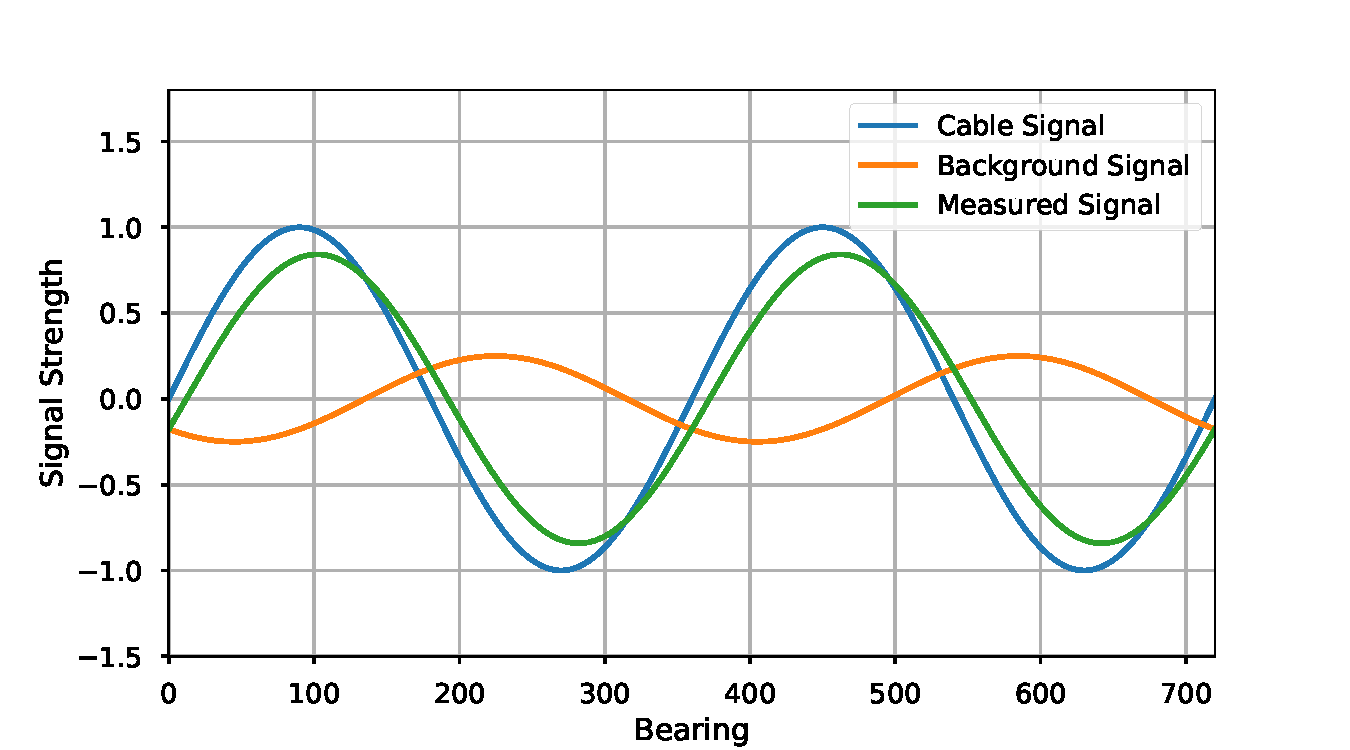
\includegraphics[width=1.0\textwidth]{figures/sigs_vs_bearing.pdf}
\end{figure}

\begin{figure}
  \caption{
  The phasor representation of the example model from Figure \ref{fig:sigs_vs_bearing}. $s$ is the measured cable signal, $b$ the background phasor and $m$ the measured phasor.  The value we really care about is $\theta$, the angle between the measured and cable signals.  Note that we can only determine the magnitude of the angle, but not the sign.  The phasor relationships shown in solids lines are indistinguishable from those shown by the dashed lines.  This model provides no information for distinguishing between the $\pm\theta$ solutions}
  \label{fig:phasor_base}
  \centering
  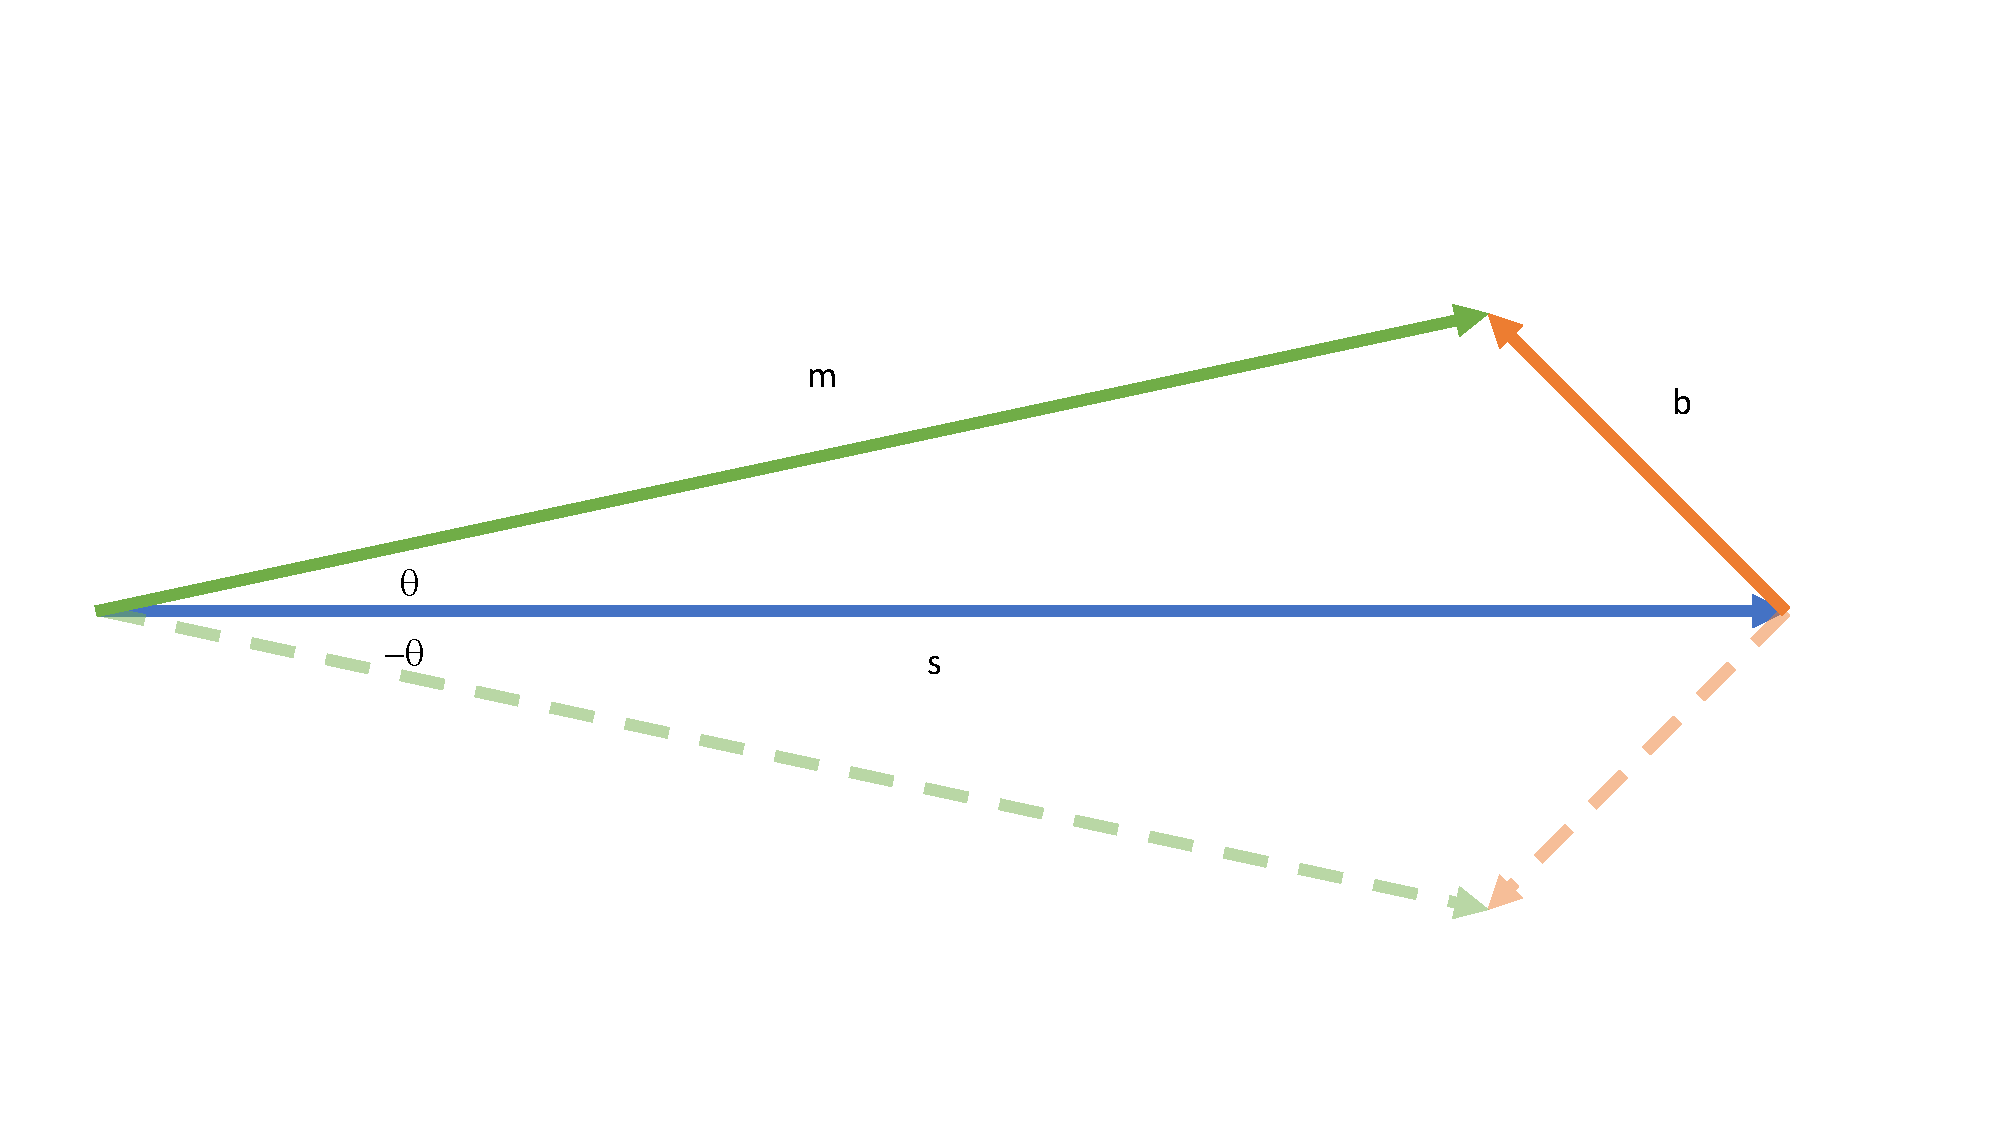
\includegraphics[width=1.0\textwidth]{figures/phasor_base.pdf}
\end{figure}

\par Our objective is to find the bearing correction that must be applied to the measured signal in order to arrive at the true cable signal.  This problem is most easily solved by considering the phasor representation.  Figure \ref{fig:phasor_base} shows the phasor representation for the same example model shown in Figure \ref{fig:sigs_vs_bearing}.  In this representation, the correction angle, $\theta$ is readily obtained from the law of cosines.

\begin{equation} \label{eq:law_of_cos}
    \cos\left(\theta\right) = \frac{m^2 + s^2 - b^2}{2ms}
\end{equation}
But since $\cos\left(\cdot\right)$ is an even function of its argument, we are unable to distinguish between solutions having positive and negative $\theta$.  So our solution becomes

\begin{equation} \label{eq:theta_solution}
\theta = \pm \cos^{-1}\left(\frac{m^2 + s^2 - b^2}{2ms}\right)
\end{equation}
where
\begin{align*}
        \theta &= \text{The angle between the measured and cable signals}\\
        s &= \text{cable signal amplitude.}\\
        b &= \text{background signal amplitude} \\
        m &= \text{measured signal amplitude} \\
\end{align*}



\subsection{Valid Solutions} \label{section:validity}
If the only information available from the system were the measured signal, there would be no way to uniquely identify what the correction angle.  This is because (referring to Figure \ref{fig:phasor_base}) there are infinitely many combinations of $s$, $b$, and $\theta$ that all generate exactly the same measured signal. We are not, however, free to pick any combination of $s$, $b$, and $\theta$.  The values we pick must be able to form a triangle in phasor space.  To get a feel for these constraints, we can rearrange equation \ref{eq:law_of_cos} to the form
\begin{equation}
    b^2 = m^2 + s^2 - 2 m s \cos\left(\theta\right).
\end{equation}
In this form it is easy to see that, for fixed $m$ and $s$, the value of $b$ must be in the range

\begin{equation*}
      m^2 + s^2 - 2 m s \leq b ^ 2 \leq  m^2 + s^2 + 2 m s
\end{equation*}
or
\begin{equation} \label{eq:bounds}
      \left(m-s\right)^2 \leq b ^ 2 \leq \left(m + s\right)^2.  
\end{equation}
Any combination of $m$, $s$ and $b$ that satisfy equation \ref{eq:bounds} is a valid solution to the phasor triangle and will have a unique value for $\cos\left(\theta\right)$.  But again, since $\cos\left(\cdot\right)$ is an even function, we are only able to determine $\theta$ up to a sign.
    
\section{Statistical Treatment}
The last two sections have shown that if we only know the measured signal, there are infinitely many combinations of background and cable signal strengths that could have resulted in that measurement.  This, of course, assumed we had absolutely no knowledge of how big we expected the background and cable signals to be.  We now allow ourselves to apply additional constraints to our problem by specifying a range of plausible values for the background and cable signals.  In practice, these plausibility ranges are determined by conducting calibration runs of the pipe and cable we are working with.  In the calibration runs, we can take many measurements of the pipe with no cable attached.  These measurements will give us a sense of the range we can expect for the background signal.  Similarly, we can carefully set up a calibration run where we deliberately configure the system to have negligible background.  In this configuration, we can measure different cable attachments to get a sense of the range we can expect for the cable signal.  We can characterize these ranges as being statistical distributions with a given mean, $\mu$, and standard deviation, $\sigma$. There are any number of statistical distributions we could use, but here we select the gamma distribution.  Our primary motivation for selecting the Gamma distribution is that, like the amplitudes we are modeling, it is only defined for positive values.  We could have chosen any other distribution with this property, but the Gamma distribution is well understood and widely used. 

\par Our approach will be to use a Monte-Carlo simulation for obtaining a probability distribution of the correction angle given the distributions determined by the mean and standard deviations we specify for both the expected cable and background signals.

Algorithm \ref{monte_algo} for sampling the bearing correction angle is summarized as follows.  We specify the distributions for the cable and background signals by defining their mean and standard deviations.  We then iterate the following process:  Draw samples from the cable and background distribution.  If those draws satisfy the triangle constraints, they are feasible, so compute the correction angle for them and include the result as a sample.  

By running many thousands of iterations of this simulation for a given measured signal, we can generate a histogram of the possible correction angles.  Fig. XXX shows such a histogram.

\begin{figure}
  \caption{Histogram of monte-carlo sampling}
  \label{fig:correction_hist}
  \centering
  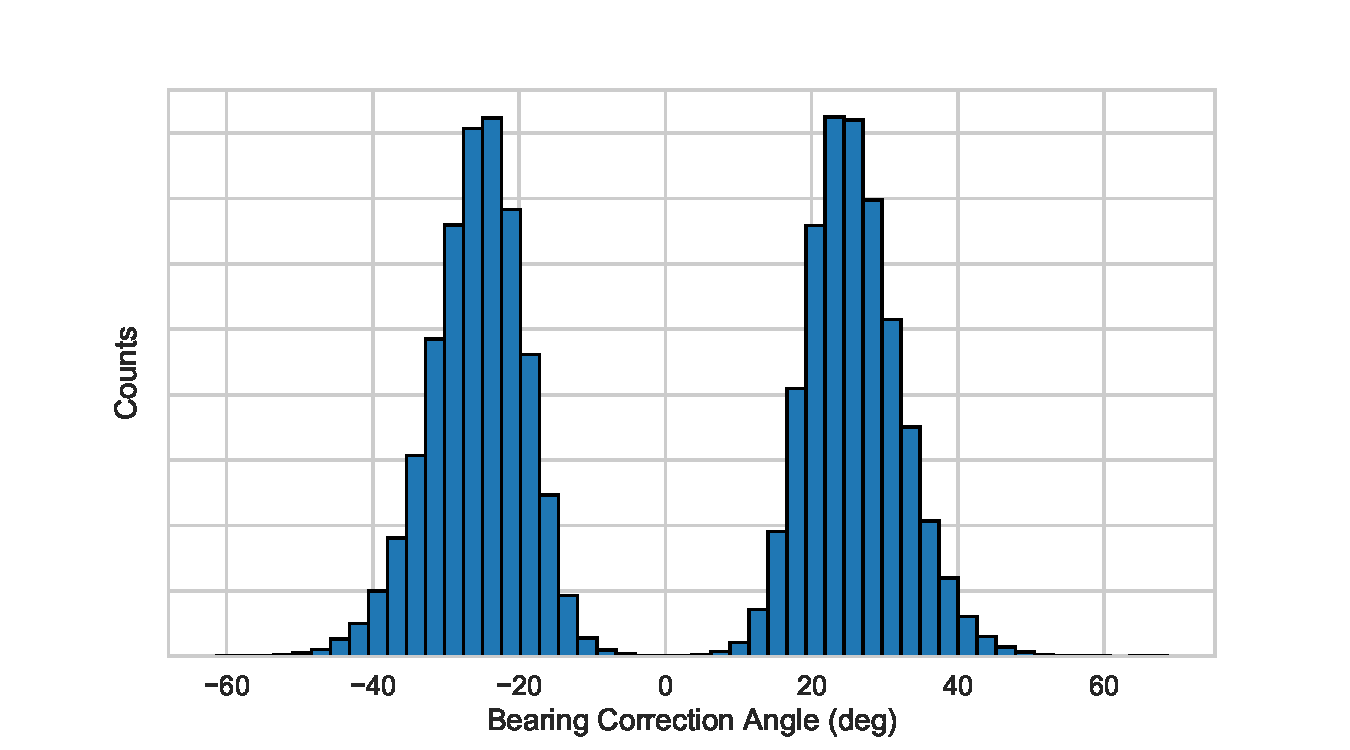
\includegraphics[width=1.0\textwidth]{figures/correction_hist.pdf}}
\end{figure}


% \lstinputlisting[language=Python]{monte_car}


\begin{algorithm}[H] \label{monte_algo}
\SetAlgoLined
\KwResult{Random samples drawn from distribution of bearing correction angles }
 $m \gets$ input the measured signal amplitude\;
 $\mu_s \gets$ input the cable signal mean\;
 $\sigma_s \gets$ input the cable signal standard deviation\;
 $\mu_b \gets$ input the background mean\;
 $\sigma_b \gets$ input the background standard deviation\;
 $N \gets$ input the desired number of samples\;
 $M \gets$ the maximum iterations for finding a triangle solution
 $n \gets 0$\;
 $\bm{\theta}} \gets$ An array of length $N$\;
 $n \gets 0$\;
 \While{n < N}{
     $i\gets0$\;
     $keepon \gets$ true\;
     \While{$i < M$ \And  keepon$}{
          $s \gets$ Draw random value from cable signal distribution\;
          $b \gets$ Draw random value from background signal distribution\;
          \uIf{$\left(m-s\right)^2 \leq b ^ 2 \leq \left(m + s\right)^2$}{
              $u \gets$ Draw randomly from $\left[-1, 1\right]$ with equal probability\; 
              $\bm{\theta}\left[n\right] \gets u \cos^{-1}\left(\frac{m^2 + s^2 - b^2}{2ms}\right)$\;
              $n = n + 1$\;
              $keepon\gets$ false\;
          }
          \Else{
              $keepon\gets$ true\;
          }
          $i \gets i + 1$\;
     }
     \If{$i = M}{
         \text{Raise an error indicating that no triangle solutions could be found}
     }

 }
 \caption{Bearing correction Monte-Carlo sampling.}
\end{algorithm}




\end{appendices}




%%% End document
\end{document}